\subsection{Labelled tokens} \label{subsection:coloring_problems}
Two prominent vertex coulouring problems that we will encounter and are part of the hardness proof of the labelled sliding token problem
are defined hereunder :

\subsubsection{$k$-colouring.}
For a positive integer $k$ and a graph $G$, we define the $k$-colour graph of $G$, denoted $\mathcal{C}_{k}(G)$,
as the graph that has the $k$-colourings of $G$ as its node set, with two $k$-colourings joined by an edge in $\mathcal{C}_{k}(G)$ if they differ
in colour on just one vertex of $G$. The $k$-COLOUR PATH is then defined as follows :
\begin{flushleft}
    k-COLOUR PATH \\
    \textbf{Instance: } Graph $G$, two $k$-colourings of $G, \alpha$ and $\beta$. \\
    \textbf{Question: } Is there a path between $\alpha$ and $\beta$ in $\mathcal{C}_{k}(G)$ ? \\
\end{flushleft}

\subsubsection{List colouring}
Suppose that we are given a graph $G=(V,E)$, and for each vertex of $G$, a list of colours permitted at that particular vertex.
In this context, the LIST-COLOUR PATH is defined as follows :
\begin{flushleft}
    LIST-COLOUR PATH \\
    \textbf{Instance: } Graph $G$, colour lists $L(v) \subseteq \{1,2,3,4\} \forall v \in V(G)$, two list-colourings $\alpha$ and $\beta$. \\
    \textbf{Question: } Is there a path between $\alpha$ and $\beta$ in $\mathcal{C}(G,L)$ ? \\
\end{flushleft}

An interesting relationship between the COLOUR-PATH problem and $k$-COLOUR PATH problem given by Bonsma is defined in lemma \ref{lemma:k_colour_to_list}.
\begin{lemma}\cite{bonsma}\label{lemma:k_colour_to_list}
For any $k \geq 4$, a LIST-COLOUR PATH instance $G, L, \alpha, \beta$ with lists $L(v) \subseteq \{1, 2, 3, 4\}$ can be transformed
into a $k$-COLOUR PATH instance $G^{'}, \alpha^{'}, \beta^{'}$ such that the distance between $\alpha$ and $\beta$ in $\mathcal{C}(G, L)$
(possibly infinite) is the same as the distance between $\alpha^{'}$ and $\beta^{'}$ in $\mathcal{C}_k(G^{'})$.
\end{lemma}

In \cite{bonsma}, Bonsma established that $k$-Colour Path is $\PSPACE$-complete for several graph classes and values of $k \geq 4$.
This result was obtained through a reduction from the Standard Sliding Token problem and done in two steps. First from the Standard
sliding token problem to the LIST-COLOUR path problem and then from the LIST-COLOUR path problem to the $k$-COLOUR path through lemma
\ref{lemma:k_colour_to_list}. In the following sections we will show that the hardness result remains even when the tokens in the
Standard sliding token instance are attributed unique labels.

\subsection{Preliminaries}
\paragraph{(a,b)-forbidding paths} For $a, b \in \{1, \dots, 4\}$,  an $(a, b)$-forbidding path from vertex $u$ to vertex $v$ is a
$(u, v)$-path with colour lists $L$, with $L(u), L(v) \neq \{1, 2, 3, 4\}$, such that in any colouring, it is not possible that
$u$ has colour $a$ and $v$ simultaneously has colour $b$ (please refer to \cite{bonsma} for the formal definition of (a,b)-forbidding paths).


\subsection{Reduction Structure}
Given a restricted instance $G, T_{A}, T_{B}, T$ of the Standard Sliding Token problem where $T$ is a set of labelled token (an example is
shown in figure \ref{fig:input_instance_standard}), we construct an instance $G^{'}, L, \alpha, \beta, T$ of LIST-COLOUR Path such that
standard token configurations of $G$ correspond to list-colourings of $G^{'}$ , and sliding a token in $G$ corresponds to a
sequence of vertex recolourings in $G^{'}$.

We first start by labelling the vertices of $G$:
\begin{enumerate}
    \item The token triangles are labelled $1, \dots , n_{t}$ , and the vertices of each triangle $i$ are labelled
    $t_{i1}$, $t_{i2}$ and $t_{i3}$.
    \item The token edges are labelled $1, \dots , n_{e}$, and the vertices of each token edge $i$ are labelled
    $e_{i1}$ and $e_{i2}$.
\end{enumerate}

The construction of $G^{'}$ is as follows: For every token triangle $i$ in $G$ we introduce a vertex $t_{i}$, with colour list
$L(t_{i}) = \{1, 2, 3\}$ in $G^{'}$ . For every token edge $i$ in $G$ we introduce a vertex $e_{i}$ in $G^{'}$, with colour
list $L(e_{i}) = \{1, 2\}$. Whenever a link edge of $G$ joins a vertex $t_{ia}$ with a vertex $e_{jb}$, we add an $(a, b)$-forbidding
path of even length between $t_{i}$ and $e_{j}$ in $G$ . We do the same for pairs $t_{ia}$ and $t_{jb}$, and pairs $e_{ia}$ and $e_{jb}$.
Linking the vertices in $G^{'}$ through $(a, b)$-forbidding paths will make sure that no tokens are adjacent to each other (an example is
shown in figure \ref{fig:output_instance_standard}). Note that this is a polynomial-time transformation.

Standard token configurations of $G$ now correspond to colourings of $G^{'}$ as follows:
\begin{enumerate}
    \item For each token edge $i$ of the token configuration, the token being on $e_{ij} (j = 1, 2 )$
    corresponds to colourings of $G$ where $e_{i}$ has colour $j$.
    \item For each token triangle $i$ of the token configuration, the token being on $t_{ij} (j = 1, 2, 3)$,
    corresponds to colourings where $t_{i}$ has colour $j$.
\end{enumerate}

Since tokens are not adjacent, it is possible to choose colours for the internal vertices of the $(a, b)$-forbidding paths so as to
obtain a proper colouring of $G^{'}$. Two colourings $\alpha$ and $\beta$ corresponding to $T_{A}$ and $T_{B}$ respectively are constructed
this way. Note that to a given standard token configuration of $G$ there can correspond multiple colourings of $G$ because of the freedom
in choice of colours for the internal vertices of the $(a, b)$-forbidding paths.

For the labels, let $W$ be the set of token edges and token triangles of $G$ i.e., $W = \{e_1,\dots, e_{|E|} \} \cup \{t_1,\dots, t_{|T|} \}$
where $|E|$ is the total number of edge tokens in $G$ and $|T|$ is the total number of triangle tokens in $G$
and $f: T \rightarrow W$, a function mapping the set of given labels to the tokens on token edges and token triangles of $G$.

\begin{claim} Let $G, T_A, T_B$ be a restricted instance of Sliding Tokens where each token is given a unique label as described in
section \ref{sec:labelled_sliding_token}, and let $G , L, \alpha, \beta$ be the corresponding instance of List-Colour Path as constructed above.
Then $G, T_A, T_B$ is a Yes-instance if and only if $G , L, \alpha, \beta$ is a YES-instance.
\end{claim}\label{theorem:labelled_sliding}

\begin{proof} \cite{bonsma}
Recall that a token configuration in which the token of token edge $i$ (token triangle $i$) is on $e_{ij}$ (on $t_ {ij}$) corresponds
to multiple colourings of $G$ where $ei$ ($t_i$) has colour $j$. Because of this multiplicity of colourings, we define colour classes of
colourings: if two colourings $\kappa$ and $\lambda$ of $G$ have $\kappa(t_i) = \lambda(t_i)$ and $\kappa(e_i) = \lambda(e_i)$ for every $i$,
then $\kappa$ and $\lambda$ are said to be in the same colour class.

Hence the correspondence between standard token configurations and colourings defines a mapping between standard
token configurations and colour classes. This mapping is in fact a bijection: $(a, b)$-forbidding paths restrict their end vertices
from having colours $a$ and $b$ respectively, but they pose no other restriction on the possible colours of their end vertices.
So $t_{ia}$ and $e_{jb}$ cannot both be occupied by a token in a token configuration if and only if no colouring $\kappa$ has $\kappa(t_i)$ = $a$
and $\kappa(e_j) = b$. (Similar statements hold for pairs $t_i$ and $t_j$, and pairs $e_i$ and $e_j$.)

The function $f$ also yields a bijective mapping : Since no token can slide along a link edge in the Standard sliding token,
each element $w \in W$ can be attributed a label such that the colour of $w$ in the output LIST-COULOUR path instance represents
the vertex placement of the label $t \in T$ s.t $f(t) = w$.

Now we claim that if there exists a sequence of moves that transforms $T_A$ into $T_B$, then there exists a sequence of
recolourings that transforms $\alpha$ into $\beta$. We mentioned earlier that any token configuration obtainable from $T_A$ is a standard
token configuration \cite{bonsma}. Hence every token move corresponds to recolouring a vertex $t_i$ or a vertex $e_i$. Note that before
recolouring $t_i$ (or $e_i$), it may be necessary to first recolour some internal vertices of $(a, b)$-forbidding paths incident with
$t_i$ (or $e_i$), but by the definition of $(a, b)$-forbidding paths, we know this is always possible. It can also be seen that when
we finally arrive in the colour class that contains $\beta$ in this way, the internal vertices of all $(a, b)$-forbidding paths can be
recoloured so that exactly the colouring $\beta$ is obtained.

Similarly, for every sequence of recolourings from $\alpha$ to $\beta$ we can construct a sequence of token moves from $T_A$ to $T_B$:
whenever a vertex $t_i$ ($e_i$) is recoloured from colour a to colour $b$, we move the corresponding token from $t_{ia}$ to $t_{ib}$
(from $e_ {ia}$ to $e_{ib}$). This completes the proof.
\end{proof}

\begin{example}{STANDARD SLIDING TOKEN problem to COLOUR-PATH reduction. \\}
    \textbf{Instance instance : STANDARD SLIDING TOKEN instance.} \hfill

    \begin{figure}[H]
        \centering
        \begin{subfigure}[b]{0.4\textwidth}
            \begin{scaletikzpicturetowidth}{\textwidth}
                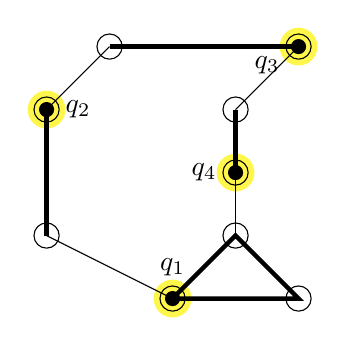
\begin{tikzpicture}[scale=0.8]
                    \def\ver{0.12} %size of a vertex
                    \def\xa{0}
                    \def\ya{0}
                    % Highlight change
                    \draw[fill=yellow, opacity=.7, draw=none] (\xa-1,\ya-1)  circle (0.3cm);
                    \draw[fill=yellow, opacity=.7, draw=none] (\xa-3,\ya+2) circle (0.3cm);
                    \draw[fill=yellow, opacity=.7, draw=none] (\xa+1,\ya+3)  circle (0.3cm);
                    \draw[fill=yellow, opacity=.7, draw=none] (\xa,\ya+1)  circle (0.3cm);
                    %graph G
                    \draw (\xa,\ya) circle (0.2cm);          % t11 no fill
                    \draw (\xa+1,\ya-1) circle (0.2cm);      % t12 no fill
                    \draw (\xa-1,\ya-1) circle (0.2cm);      % t13 no fill
                    \draw (\xa-3,\ya) circle (0.2cm);        % e11 no fill
                    \draw (\xa-3,\ya+2) circle (0.2cm);      % e12 no fill
                    \draw (\xa-2,\ya+3) circle (0.2cm);      % e21 no fill
                    \draw (\xa+1,\ya+3) circle (0.2cm);      % e22 no fill
                    \draw (\xa,\ya+2) circle (0.2cm);        % e31 no fill
                    \draw (\xa,\ya+1) circle (0.2cm);        % e32 no fill
                    % Tokens
                    \path[fill] (\xa-1,\ya-1) circle (\ver);   % t13
                    \path[fill] (\xa-3,\ya+2) circle (\ver);   % e12
                    \path[fill] (\xa+1,\ya+3) circle (\ver);   % e22
                    \path[fill] (\xa,\ya+1) circle (\ver);     % e32
                    % edges
                    \draw[ultra thick] (\xa,\ya)--(\xa+1,\ya-1)--(\xa-1,\ya-1)--cycle;
                    \draw[ultra thick] (\xa-3,\ya)--(\xa-3,\ya+2) ;
                    \draw[ultra thick] (\xa-2,\ya+3)--(\xa+1,\ya+3) ;
                    \draw[ultra thick] (\xa,\ya+2)--(\xa,\ya+1) ;
                    \draw (\xa-2,\ya+3)--(\xa-3,\ya+2);
                    \draw (\xa-3,\ya)--(\xa-1,\ya-1);
                    \draw (\xa,\ya+1)--(\xa,\ya);
                    \draw (\xa,\ya+2)--(\xa+1,\ya+3);
                    % token labels
                    \node (l1) at (\xa-1,\ya-0.5) {$q_{1}$};            % Label
                    \node (l2) at (\xa-2.5,\ya+2) {$q_{2}$};            % Label
                    \node (l3) at (\xa+0.5,\ya+2.7) {$q_{3}$};            % Label
                    \node (l4) at (\xa-0.5,\ya+1) {$q_{4}$};            % Label

                \end{tikzpicture}
            \end{scaletikzpicturetowidth}
            \caption{Initial token configuration $T_{A}$.}
            \label{fig:standard_1}
        \end{subfigure}
        \begin{subfigure}[b]{0.4\textwidth}
            \begin{scaletikzpicturetowidth}{\textwidth}
                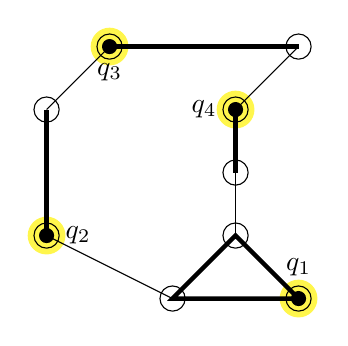
\begin{tikzpicture}[scale=0.8]
                    \def\ver{0.12} %size of a vertex
                    \def\xa{0}
                    \def\ya{0}
                    % Highlight change
                    \draw[fill=yellow, opacity=.7, draw=none] (\xa+1,\ya-1)  circle (0.3cm);
                    \draw[fill=yellow, opacity=.7, draw=none] (\xa-3,\ya) circle (0.3cm);
                    \draw[fill=yellow, opacity=.7, draw=none] (\xa-2,\ya+3)  circle (0.3cm);
                    \draw[fill=yellow, opacity=.7, draw=none] (\xa,\ya+2)  circle (0.3cm);
                    %graph G
                    \draw (\xa,\ya) circle (0.2cm);          % t11 no fill
                    \draw (\xa+1,\ya-1) circle (0.2cm);      % t12 no fill
                    \draw (\xa-1,\ya-1) circle (0.2cm);      % t13 no fill
                    \draw (\xa-3,\ya) circle (0.2cm);        % e11 no fill
                    \draw (\xa-3,\ya+2) circle (0.2cm);      % e12 no fill
                    \draw (\xa-2,\ya+3) circle (0.2cm);      % e21 no fill
                    \draw (\xa+1,\ya+3) circle (0.2cm);      % e22 no fill
                    \draw (\xa,\ya+2) circle (0.2cm);        % e31 no fill
                    \draw (\xa,\ya+1) circle (0.2cm);        % e32 no fill
                    % Tokens
                    \path[fill] (\xa+1,\ya-1) circle (\ver);   % t12
                    \path[fill] (\xa-3,\ya) circle (\ver);     % e11
                    \path[fill] (\xa-2,\ya+3) circle (\ver);   % e21
                    \path[fill] (\xa,\ya+2) circle (\ver);     % e31
                    % edges
                    \draw[ultra thick] (\xa,\ya)--(\xa+1,\ya-1)--(\xa-1,\ya-1)--cycle;
                    \draw[ultra thick] (\xa-3,\ya)--(\xa-3,\ya+2) ;
                    \draw[ultra thick] (\xa-2,\ya+3)--(\xa+1,\ya+3) ;
                    \draw[ultra thick] (\xa,\ya+2)--(\xa,\ya+1) ;
                    \draw (\xa-2,\ya+3)--(\xa-3,\ya+2);
                    \draw (\xa-3,\ya)--(\xa-1,\ya-1);
                    \draw (\xa,\ya+1)--(\xa,\ya);
                    \draw (\xa,\ya+2)--(\xa+1,\ya+3);
                    % token labels
                    \node (l1) at (\xa+1,\ya-0.5) {$q_{1}$};            % Label (\xa+1,\ya-1)
                    \node (l2) at (\xa-2.5,\ya) {$q_{2}$};            % Label (\xa-3,\ya)
                    \node (l3) at (\xa-2,\ya+2.6) {$q_{3}$};            % Label (\xa-2,\ya+3)
                    \node (l4) at (\xa-0.5,\ya+2) {$q_{4}$};            % Label (\xa,\ya+2)
                \end{tikzpicture}
            \end{scaletikzpicturetowidth}
            \caption{Target token configuration $T_{B}$.}
            \label{fig:standard_2}
        \end{subfigure}
        \caption{A Standard sliding token instance with initial and target labelled token configuration $T_{A}$ and $T_{B}$ respectively.}
        \label{fig:input_instance_standard}
    \end{figure}

% ------------------------- Output instance 1 -----------------------------
    \textbf{Output instance : LIST-COLOUR path instance.} \hfill
    \begin{figure}[H]
        \begin{subfigure}[b]{0.9\textwidth}
            \begin{scaletikzpicturetowidth}{\textwidth}
                \begin{tikzpicture}[scale=0.8]
                    \centering
                    \def\ver{0.12} %size of a vertex
                    \def\xa{0}
                    \def\ya{0}
                    \node[Bullet=purple,label=above :{$\{1,2,3\}$}] (t1) at (\xa,\ya+3){};             % t1
                    \node[Bullet=blue,label=left :{$\{1,3\}$}] (t11) at (\xa-3,\ya+1.5){};             % t11
                    \node[Bullet=blue,label=right:{$\{2,1\}$}] (e33) at (\xa+1.5,\ya+2.2){};           % e33
                    \node[Bullet=green,label=right:{$\{2,3\}$}] (e32) at (\xa+3,\ya+1.5){};            % e32
                    \node[Bullet=purple,label=right:{$\{3,2\}$}] (e31) at (\xa+4.5,\ya+0.8){};         % e31
                    \node[Bullet=green,label=below :{$\{1,2\}$}] (e3) at (\xa+6,\ya){};                % e3
                    \node[Bullet=blue,label=below :{$\{3,1\}$}] (e23) at (\xa+4.5,\ya){};              % e23
                    \node[Bullet=purple,label=below :{$\{1,3\}$}] (e22) at (\xa+3,\ya){};              % e22
                    \node[Bullet=blue,label=below :{$\{1,2\}$}] (e21) at (\xa+1.5,\ya){};              % e21
                    \node[Bullet=green,label=above :{$\{1,2\}$}] (e2) at (\xa,\ya){};                  % e2
                    \node[Bullet=blue,label=below :{$\{3,1\}$}] (e13) at (\xa-1.5,\ya){};              % e13
                    \node[Bullet=purple,label=below :{$\{1,3\}$}] (e12) at (\xa-3,\ya){};              % e12
                    \node[Bullet=blue,label=below :{$\{1,2\}$}] (e11) at (\xa-4.5,\ya){};              % e11
                    \node[Bullet=green,label=below :{$\{1,2\}$}] (e1) at (\xa-6,\ya){};                % e1

                    \draw[thick] (e1)--(e11)--(e12)--(e13)--(e2)--(e21)--(e22)--(e23)--(e3)--(e31)--(e32)--(e33)--(t1)--(t11)--(e1);
                \end{tikzpicture}
            \end{scaletikzpicturetowidth}
            \caption{Initial colouring $\alpha$.}
            \label{fig:list_colour_1}
        \end{subfigure}
        \medskip
        \begin{subfigure}[b]{0.9\textwidth}
            \begin{scaletikzpicturetowidth}{\textwidth}
                \begin{tikzpicture}[scale=0.8]
                    \centering
                    \def\ver{0.12} %size of a vertex
                    \def\xa{0}
                    \def\ya{0}
                    \node[Bullet=green,label=above :{$\{1,2,3\}$}] (t1) at (\xa,\ya+3){};             % t1
                    \node[Bullet=purple,label=left :{$\{1,3\}$}] (t11) at (\xa-3,\ya+1.5){};          % t11
                    \node[Bullet=blue,label=right:{$\{2,1\}$}] (e33) at (\xa+1.5,\ya+2.2){};          % e33
                    \node[Bullet=green,label=right:{$\{2,3\}$}] (e32) at (\xa+3,\ya+1.5){};           % e32
                    \node[Bullet=purple,label=right:{$\{3,2\}$}] (e31) at (\xa+4.5,\ya+0.8){};        % e31
                    \node[Bullet=blue,label=below :{$\{1,2\}$}] (e3) at (\xa+6,\ya){};                % e3
                    \node[Bullet=purple,label=below :{$\{3,1\}$}] (e23) at (\xa+4.5,\ya){};           % e23
                    \node[Bullet=blue,label=below :{$\{1,3\}$}] (e22) at (\xa+3,\ya){};               % e22
                    \node[Bullet=green,label=below :{$\{1,2\}$}] (e21) at (\xa+1.5,\ya){};            % e21
                    \node[Bullet=blue,label=above :{$\{1,2\}$}] (e2) at (\xa,\ya){};                  % e2
                    \node[Bullet=purple,label=below :{$\{3,1\}$}] (e13) at (\xa-1.5,\ya){};           % e13
                    \node[Bullet=blue,label=below :{$\{1,3\}$}] (e12) at (\xa-3,\ya){};               % e12
                    \node[Bullet=green,label=below :{$\{1,2\}$}] (e11) at (\xa-4.5,\ya){};            % e11
                    \node[Bullet=blue,label=below :{$\{1,2\}$}] (e1) at (\xa-6,\ya){};                % e1

                    \draw[thick] (e1)--(e11)--(e12)--(e13)--(e2)--(e21)--(e22)--(e23)--(e3)--(e31)--(e32)--(e33)--(t1)--(t11)--(e1);
                \end{tikzpicture}
            \end{scaletikzpicturetowidth}
            \caption{Target colouring $\beta$}
            \label{fig:list_colour_2}
        \end{subfigure}
        \caption{Output LIST-COLOUR path instance with $\alpha$ being the initial colouring and $\beta$ the target colouring where for better
        visualisation the colour blue is associated to 1, green to 2 and purple to 3 .}
        \label{fig:output_instance_standard}
    \end{figure}
\end{example}